
\documentclass[border=10pt]{standalone}

\usepackage{tikz}
\usetikzlibrary{fit,positioning,calc}


%default strings

\begin{document}
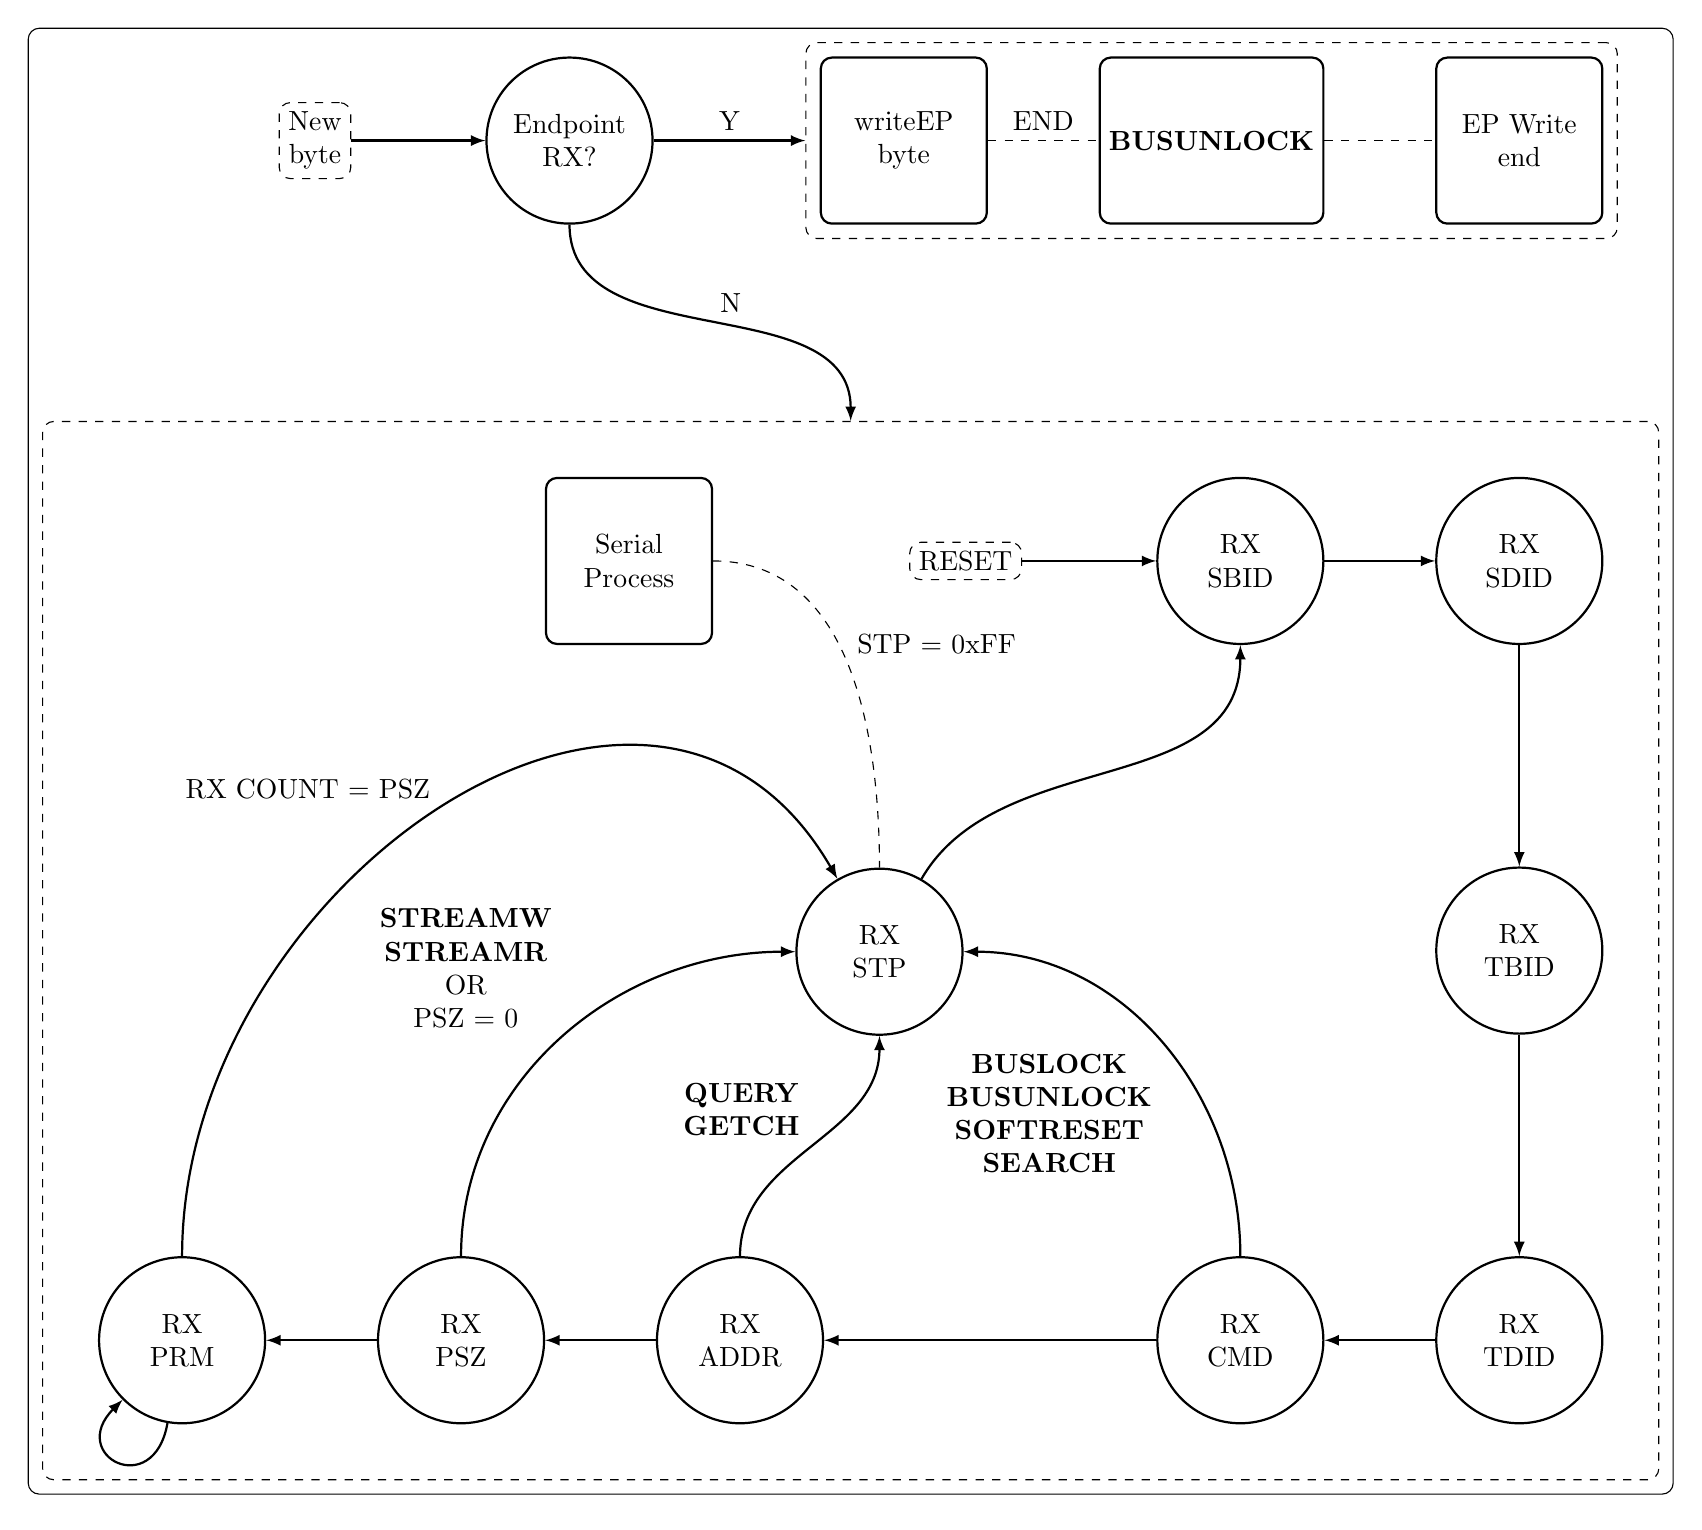
\begin{tikzpicture}[auto]

\tikzstyle{stackitem}=[rounded corners,align=center,thick,circle,minimum size=60pt,draw=black, node distance=40pt]
\tikzstyle{process}=[rounded corners,align=center,thick,rectangle,minimum size=60pt,draw=black, node distance=20pt]

\node [stackitem] (eprx) {Endpoint \\ RX?};

\node [process,right= of eprx, xshift=40pt] (ep1) {writeEP \\ byte};
\node [process,right= of ep1,xshift=20pt] (ep2) {\textbf{BUSUNLOCK}};
\node [process,right= of ep2,xshift=20pt] (ep3) {EP Write \\ end};

\path [dashed] (ep1) edge node {END} (ep2)
      (ep2) edge (ep3);

\node [draw=black,rounded corners,dashed,fit= (ep1) (ep2) (ep3),inner sep=5pt] (epx) {};

\path [-latex,thick] (eprx) edge node {Y} (epx);

\node [dashed,rounded corners,draw=black,left= of eprx,xshift=-20pt,align=center] (newbyte) {New \\ byte};
\path [-latex,thick] (newbyte) edge (eprx);


\node [process,below= of eprx.south east,yshift=-80pt] (sproc) {Serial \\ Process};
\node [stackitem] (sdid) at (sproc -| ep3) {RX \\ SDID};
\node [stackitem,left= of sdid] (sbid) {RX \\ SBID};
\node [stackitem,below= of sdid,yshift=-40pt] (tbid) {RX \\ TBID};
\node [stackitem,below= of tbid,yshift=-40pt] (tdid) {RX \\ TDID};

\node [stackitem,left= of tdid] (cmd) {RX \\ CMD};
\node [stackitem,left= of cmd,xshift=-80pt] (addr) {RX \\ ADDR};
\node [stackitem,left= of addr] (psz) {RX \\ PSZ};
\node [stackitem,left= of psz] (prm) {RX\\ PRM};

\node [stackitem,above= of addr.east,yshift=70pt,xshift=20pt] (stp) {RX \\ STP};

\node [draw=black,rounded corners,dashed, left= of sbid,xshift=-20pt] (reset) {RESET};

\path [-latex,thick] (reset) edge (sbid)
      (sbid) edge (sdid)
      (sdid) edge (tbid)
      (tbid) edge (tdid)
      (tdid) edge (cmd)
      (cmd) edge (addr)
      (addr) edge (psz)
      (psz) edge (prm)
      (prm) edge [out=260,in=225,looseness=4] (prm)
      (cmd) edge [out=90,in=0] node [align=center,font=\bf] {BUSLOCK \\ BUSUNLOCK \\ SOFTRESET \\ SEARCH} (stp)
      (addr) edge [out=90,in=270] node [align=center,font=\bf] {QUERY \\ GETCH} (stp)
      (psz) edge [out=90,in=180] node [align=center] {\bfseries STREAMW \\ \bfseries STREAMR \\ OR \\ PSZ = 0} (stp)
      (stp) edge [out=60,in=270] (sbid)
      (prm) edge [out=90,in=120,looseness=1.25] node {RX COUNT = PSZ} (stp);

\path [dashed] (sproc) edge [out=0,in=90] node {STP = 0xFF} (stp);

\node [dashed,rounded corners,draw=black,fit= (sproc) (prm) (tdid),inner sep=20pt] (states) {};
\path [-latex,thick] (eprx) edge [out=270,in=90] node {N} (states);

\node [draw=black,rounded corners, fit= (states) (epx),inner sep=5pt] {};

\end{tikzpicture}
\end{document}